% TEX root = ../main.tex
\section{Diseño}

\subsection{Planteamiento de circuito}

Para conectar los distintos periféricos que se van a utilizar, se dispuso el
circuito tal como se observa en la \autoref{fig:diag-circuito}. En primer
lugar, cada módulo debe ser energizado, y para esto se utilizaron
principalmente los pines de \texttt{+5V} y \texttt{GND} del Arduino UNO, a
excepción del display Nextion, el cual, debido a que el Arduino puede
suministrar sólamente hasta $700\ \unit{mA}$ de corriente, lo cual era
insuficiente para el display, por lo que se utilizó alimentación externa
mediante una placa con un conector USB Micro-B.

\begin{figure}[ht]
    \centering
    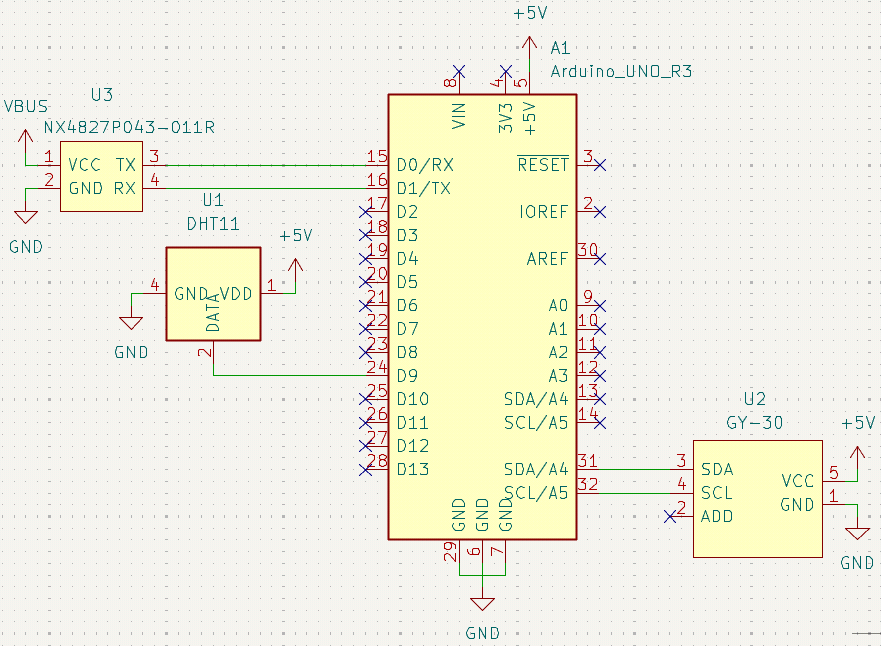
\includegraphics[width=0.75\textwidth]{Diagramas/circuito.png}
    \caption{}\label{fig:diag-circuito}
\end{figure}

Luego, para la comunicación de los distintos periféricos con el Arduino, se
utilizaron distintos métodos. En primer lugar, el módulo DHT-11 utiliza un
protocolo de comunicación bidireccional con un sólo cable, el cual se conectó a
un pin digital del Arduino, específicamente el pin \texttt{D9}. Luego, el
sensor de luminosidad GY-30, utiliza protocolo de comunicación I2C, por lo que
se conecta el pin \texttt{SDA} del módulo al \texttt{SDA/A4} del Arduino, y el
pin \texttt{SCL} del módulo al \texttt{SCL/A5} del Arduino. Finalmente, el
la pantalla HMI utiliza comunicación mediante TTL serial, por lo que se conecta
el \texttt{TX} del HMI a \texttt{D0/RX} del Arduino, y \texttt{RX} del display
a \texttt{D1/TX}.

\subsection{Desarrollo del código}

Una vez definida la conexión de los periféricos al Arduino, se procedió
al desarrollo del código. Como se puede observar en el \autoref{lst:codigo-1},
se empieza por importar varios headers, los cuales contienen las definiciones
de las librerías que se van a utilizar, siendo estas:
\begin{itemize}
    \item \texttt{Wire.h}: utilizada para comunicación I2C con el sensor de luminosidad.
    \item \texttt{DHT.h}: utilizada para comunicación con sensor de temperatura y humedad.
    \item \texttt{BH1750.h}: funciones que facilitan la comunicación con el sensor de luminosidad.
    \item \texttt{Nextion.h}: para comunicación con HMI Nextion.
\end{itemize}

Luego, se tienen definiciones de los objetos que se utilizará para comunicarse
con los periféricos. En primer lugar entonces se define el tipo de sensor DHT
que se va a utilizar, en este caso es DHT-11, y a cuál pin se tiene conectado
el pin de datos de este. Luego, utilizando estas definiciones, se instancia el
objeto para DHT. A continuación se instancia igualmente el objeto para el sensor
de luminosidad.

A continuación se tiene la función \texttt{setup}, la cual es ejecutada una sola
vez al encender el Arduino, o luego de un Reset. Aquí se comienza por inicializar
comunicación serial a 9600 baudios para comunicarse con el HMI. Luego, se llama
al método \texttt{begin} del objeto DHT para que se configure todo lo necesario
para la comunicación con este. Además, se inicializa la librería para el display
Nextion, para comunicación por I2C mediante la librería \texttt{Wire} y finalmente
la comunicación con el sensor de luminosidad.

Entonces, se procede a la función \texttt{loop}, la cual se ejecuta repetidas
veces luego de que se haya ejecutado \texttt{setup}, hasta que el Arduino
pierda energía, o este se reinicie. Se comienza entonces con un delay de $100\
\unit{ms}$, lo cual será la velocidad de muestreo de los sensores, y entonces
se procede a leer los valores reportados por estos, haciendo llamado a los
distintos métodos proporcionados por las librerías. Con estos valores, se
procede entonces a enviar la información a la pantalla Nextion. Para esto, se
crean objetos \texttt{String} y se transforman los valores leidos a cadenas de
caracteres. Luego, se envían los datos, concatenando estos con el nombre del
campo de texto correspondiente. Para la temperatura, fue necesario utilizar el
código ASCII del símbolo de grado ($^{\circ}$) puesto que, probablemente debido
a que el display y el código fuente de Arduino utilizan codificaciones de texto
distintas, escribir el símbolo directamente ocasinaba que símbolos adicionales
aparecieran en la pantalla. Para el resto de las variables, se utilizó la
función \texttt{enviarComando} que simplemente utiliza la comunicación serial
para enviar el string concatendado que se le entrega y luego se hace llamado
a \texttt{terminarComando} que envía los bytes de terminación a la pantalla
para denotar que ya se enviaron los datos.

Luego, se tiene el envío de datos para el despliegue mediante gráficos en
la interfaz. Para esto, se empieza por instanciar un objeto de tipo
\texttt{NexWaveform}, asignándole un ID de página, ID de componente y
nombre. Luego, se mapea el valor a al rango admitido por el HMI, que
es entre $0-255$, a continuación, con la función \texttt{constraint} se
asegura que el valor no se salga de este rango, y finalmente se envía el
valor al HMI mediante el método \texttt{addValue}.

\clearpage
\subsection{Diseño de interfaz}

Para el diseño de la interfaz grafica, se utilizaron 2 herramientas. Siendo la principal
\texttt{Nextion Editor}, debido a que aqui se declaraban los distintos elementos para 
cumplir con los requerimientos del laboratorio. En este caso se ideo que se mostraran 
los valores de humedad, temperatura y luminosidad. Junto a un grafico que dependiendo 
que valor se presionara mostrara la evolucion en el tiempo del elemento seleccionado.
Ubicando botones encima del texto para mostrar los valores, se logro que la interfaz 
cambiara al presionar los distintos valores.
\begin{figure}[h!]
    \centering
    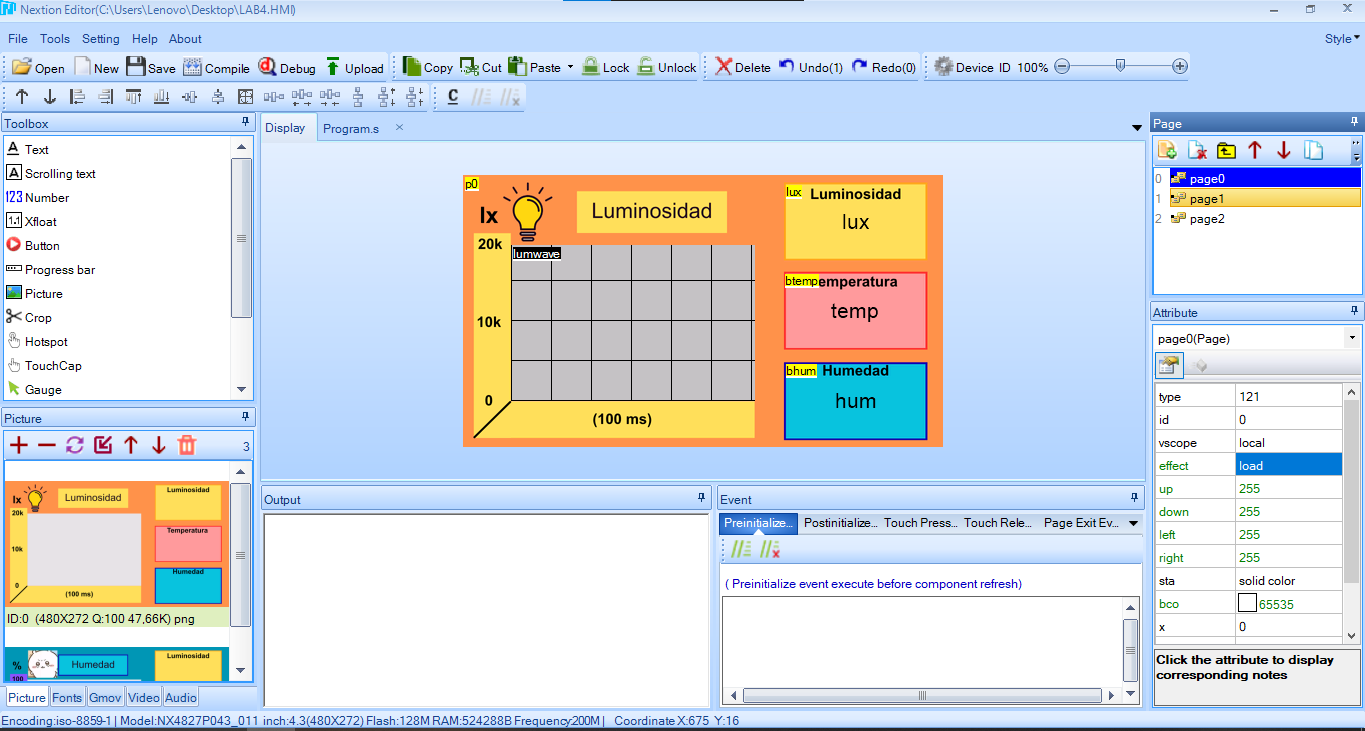
\includegraphics[width=0.8\textwidth]{Diagramas/nextion.png}
    \caption{Programa \texttt{Nextion}}
    \label{fig:nextion}
\end{figure}

Como segundo programa, se utilizo \texttt{Canva}.
Este se uso principalmente para el diseño de la interfaz, sirviendo de plantilla para 
ubicar los botones y graficos. Agregando colores e imagenes que esten relacionadas 
con el valor medido. Logrando las siguientes interfaces.

\begin{figure}[h!]
    \centering

    % --- Fila superior: dos imágenes centradas ---
    \begin{subfigure}[t]{0.45\textwidth}
        \centering
        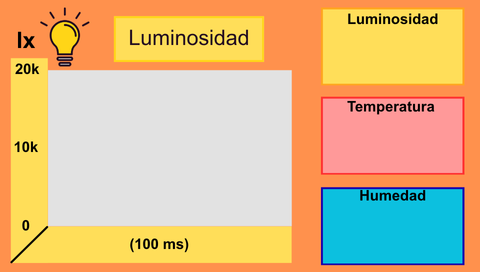
\includegraphics[width=\textwidth]{Diagramas/1.png}
        \caption{Interfaz para luminosidad.}
        \label{fig:sub1}
    \end{subfigure}
    \hfill
    \begin{subfigure}[t]{0.45\textwidth}
        \centering
        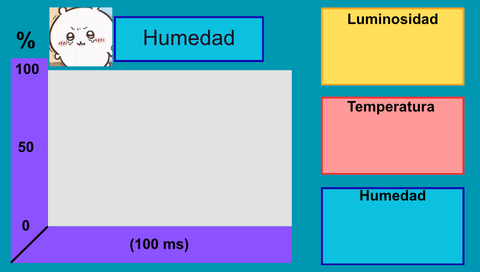
\includegraphics[width=\textwidth]{Diagramas/2.png}
        \caption{Interfaz para humedad.}
        \label{fig:sub2}
    \end{subfigure}
    
    % --- Espacio entre filas ---
    \vskip1em
    
    % --- Fila inferior: una imagen centrada ---
    \begin{subfigure}[t]{0.45\textwidth}
        \centering
        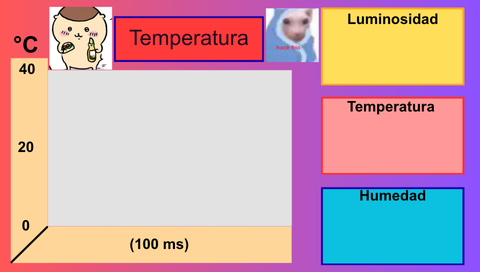
\includegraphics[width=\textwidth]{Diagramas/3.png}
        \caption{Interfaz para temperatura.}
        \label{fig:sub3}
    \end{subfigure}

    \caption{Interfaces desarrolladas en \texttt{Canva}.}
    \label{fig:tres_imagenes}
\end{figure}
